\documentclass[twoside]{book}

% Packages required by doxygen
\usepackage{fixltx2e}
\usepackage{calc}
\usepackage{doxygen}
\usepackage[export]{adjustbox} % also loads graphicx
\usepackage{graphicx}
\usepackage[utf8]{inputenc}
\usepackage{makeidx}
\usepackage{multicol}
\usepackage{multirow}
\PassOptionsToPackage{warn}{textcomp}
\usepackage{textcomp}
\usepackage[nointegrals]{wasysym}
\usepackage[table]{xcolor}

% Font selection
\usepackage[T1]{fontenc}
\usepackage[scaled=.90]{helvet}
\usepackage{courier}
\usepackage{amssymb}
\usepackage{sectsty}
\renewcommand{\familydefault}{\sfdefault}
\allsectionsfont{%
  \fontseries{bc}\selectfont%
  \color{darkgray}%
}
\renewcommand{\DoxyLabelFont}{%
  \fontseries{bc}\selectfont%
  \color{darkgray}%
}
\newcommand{\+}{\discretionary{\mbox{\scriptsize$\hookleftarrow$}}{}{}}

% Page & text layout
\usepackage{geometry}
\geometry{%
  a4paper,%
  top=2.5cm,%
  bottom=2.5cm,%
  left=2.5cm,%
  right=2.5cm%
}
\tolerance=750
\hfuzz=15pt
\hbadness=750
\setlength{\emergencystretch}{15pt}
\setlength{\parindent}{0cm}
\setlength{\parskip}{3ex plus 2ex minus 2ex}
\makeatletter
\renewcommand{\paragraph}{%
  \@startsection{paragraph}{4}{0ex}{-1.0ex}{1.0ex}{%
    \normalfont\normalsize\bfseries\SS@parafont%
  }%
}
\renewcommand{\subparagraph}{%
  \@startsection{subparagraph}{5}{0ex}{-1.0ex}{1.0ex}{%
    \normalfont\normalsize\bfseries\SS@subparafont%
  }%
}
\makeatother

% Headers & footers
\usepackage{fancyhdr}
\pagestyle{fancyplain}
\fancyhead[LE]{\fancyplain{}{\bfseries\thepage}}
\fancyhead[CE]{\fancyplain{}{}}
\fancyhead[RE]{\fancyplain{}{\bfseries\leftmark}}
\fancyhead[LO]{\fancyplain{}{\bfseries\rightmark}}
\fancyhead[CO]{\fancyplain{}{}}
\fancyhead[RO]{\fancyplain{}{\bfseries\thepage}}
\fancyfoot[LE]{\fancyplain{}{}}
\fancyfoot[CE]{\fancyplain{}{}}
\fancyfoot[RE]{\fancyplain{}{\bfseries\scriptsize Generated by Doxygen }}
\fancyfoot[LO]{\fancyplain{}{\bfseries\scriptsize Generated by Doxygen }}
\fancyfoot[CO]{\fancyplain{}{}}
\fancyfoot[RO]{\fancyplain{}{}}
\renewcommand{\footrulewidth}{0.4pt}
\renewcommand{\chaptermark}[1]{%
  \markboth{#1}{}%
}
\renewcommand{\sectionmark}[1]{%
  \markright{\thesection\ #1}%
}

% Indices & bibliography
\usepackage{natbib}
\usepackage[titles]{tocloft}
\setcounter{tocdepth}{3}
\setcounter{secnumdepth}{5}
\makeindex

% Hyperlinks (required, but should be loaded last)
\usepackage{ifpdf}
\ifpdf
  \usepackage[pdftex,pagebackref=true]{hyperref}
\else
  \usepackage[ps2pdf,pagebackref=true]{hyperref}
\fi
\hypersetup{%
  colorlinks=true,%
  linkcolor=blue,%
  citecolor=blue,%
  unicode%
}

% Custom commands
\newcommand{\clearemptydoublepage}{%
  \newpage{\pagestyle{empty}\cleardoublepage}%
}

\usepackage{caption}
\captionsetup{labelsep=space,justification=centering,font={bf},singlelinecheck=off,skip=4pt,position=top}

%===== C O N T E N T S =====

\begin{document}

% Titlepage & ToC
\hypersetup{pageanchor=false,
             bookmarksnumbered=true,
             pdfencoding=unicode
            }
\pagenumbering{alph}
\begin{titlepage}
\vspace*{7cm}
\begin{center}%
{\Large Formula1 Racing Simulator }\\
\vspace*{1cm}
{\large Generated by Doxygen 1.8.13}\\
\end{center}
\end{titlepage}
\clearemptydoublepage
\pagenumbering{roman}
\tableofcontents
\clearemptydoublepage
\pagenumbering{arabic}
\hypersetup{pageanchor=true}

%--- Begin generated contents ---
\chapter{cpp\+\_\+project}
\label{autotoc_md0}
\Hypertarget{autotoc_md0}
This project was made with Jetbrain C\+L\+I\+ON 2019.\+3.\+4 use C++20 Need \+: -\/\+Visual studio 2019


\begin{DoxyItemize}
\item Open the project
\item Build the project N\+O\+M\+S\+D\+U\+P\+R\+O\+J.\+exe has been build in cmake-\/build folder
\end{DoxyItemize}

Need \+: -\/\+C\+M\+A\+KE V\+E\+R\+S\+I\+ON $>$ 3.\+15 -\/\+Visual studio 2019


\begin{DoxyItemize}
\item Use the {\ttfamily cmake .} command in the folder to compile the project
\item Open N\+O\+M\+S\+D\+U\+P\+R\+O\+J.\+sln
\item Then generate N\+O\+M\+S\+D\+U\+P\+R\+OJ N\+O\+M\+S\+D\+U\+P\+R\+O\+J.\+exe has been build in Debug folder or Release folder , it depend on which one you choosed.
\end{DoxyItemize}


\begin{DoxyItemize}
\item Pression des pneus
\item Usure des pneus
\item Température du moteur
\item Taux d\textquotesingle{}essence
\item Taux d\textquotesingle{}huile
\item Usure du systeme de freinage
\item Usure du D\+RS
\item Usure de l\textquotesingle{}antiblocage au freinage
\item Usure de la colonne de direction
\item Etat de la carroserie 
\end{DoxyItemize}
\chapter{Class Index}
\section{Class List}
Here are the classes, structs, unions and interfaces with brief descriptions\+:\begin{DoxyCompactList}
\item\contentsline{section}{\hyperlink{class_cars}{Cars} }{\pageref{class_cars}}{}
\item\contentsline{section}{\hyperlink{class_cars__bot}{Cars\+\_\+bot} }{\pageref{class_cars__bot}}{}
\item\contentsline{section}{\hyperlink{class_circuit}{Circuit} }{\pageref{class_circuit}}{}
\item\contentsline{section}{\hyperlink{class_race}{Race} }{\pageref{class_race}}{}
\item\contentsline{section}{\hyperlink{classutils}{utils} }{\pageref{classutils}}{}
\end{DoxyCompactList}

\chapter{File Index}
\section{File List}
Here is a list of all files with brief descriptions\+:\begin{DoxyCompactList}
\item\contentsline{section}{\hyperlink{main_8cpp}{main.\+cpp} }{\pageref{main_8cpp}}{}
\item\contentsline{section}{Classes/\hyperlink{_cars_8cpp}{Cars.\+cpp} }{\pageref{_cars_8cpp}}{}
\item\contentsline{section}{Classes/\hyperlink{_cars_8h}{Cars.\+h} }{\pageref{_cars_8h}}{}
\item\contentsline{section}{Classes/\hyperlink{_cars__bot_8cpp}{Cars\+\_\+bot.\+cpp} }{\pageref{_cars__bot_8cpp}}{}
\item\contentsline{section}{Classes/\hyperlink{_cars__bot_8h}{Cars\+\_\+bot.\+h} }{\pageref{_cars__bot_8h}}{}
\item\contentsline{section}{Classes/\hyperlink{_circuit_8cpp}{Circuit.\+cpp} }{\pageref{_circuit_8cpp}}{}
\item\contentsline{section}{Classes/\hyperlink{_circuit_8h}{Circuit.\+h} }{\pageref{_circuit_8h}}{}
\item\contentsline{section}{Classes/\hyperlink{_race_8cpp}{Race.\+cpp} }{\pageref{_race_8cpp}}{}
\item\contentsline{section}{Classes/\hyperlink{_race_8h}{Race.\+h} }{\pageref{_race_8h}}{}
\item\contentsline{section}{Classes/\hyperlink{utils_8cpp}{utils.\+cpp} }{\pageref{utils_8cpp}}{}
\item\contentsline{section}{Classes/\hyperlink{utils_8h}{utils.\+h} }{\pageref{utils_8h}}{}
\end{DoxyCompactList}

\chapter{Class Documentation}
\hypertarget{class_cars}{}\section{Cars Class Reference}
\label{class_cars}\index{Cars@{Cars}}


{\ttfamily \#include $<$Cars.\+h$>$}



Collaboration diagram for Cars\+:
\nopagebreak
\begin{figure}[H]
\begin{center}
\leavevmode
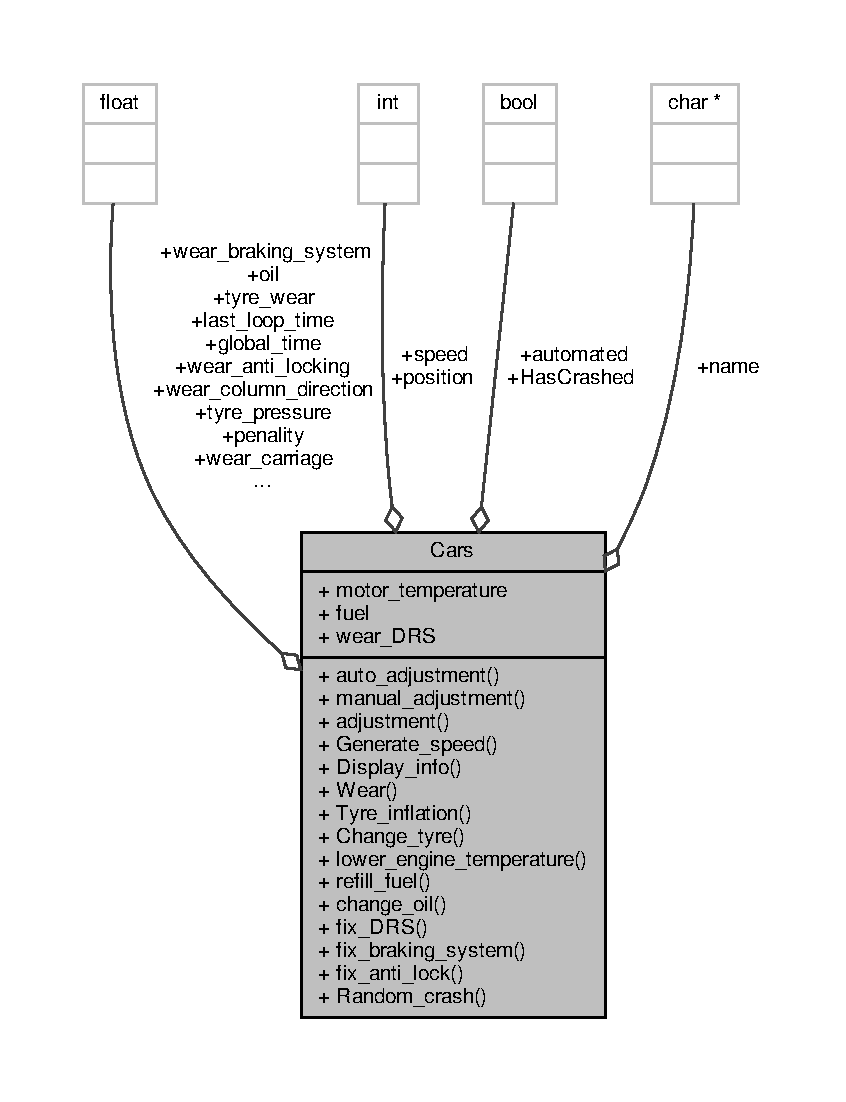
\includegraphics[width=350pt]{class_cars__coll__graph}
\end{center}
\end{figure}
\subsection*{Public Member Functions}
\begin{DoxyCompactItemize}
\item 
void \hyperlink{class_cars_ae7e733fb41d03d016dd0c7d5a047f9c9}{auto\+\_\+adjustment} ()
\item 
void \hyperlink{class_cars_a87ccc17a207f38be7181636757e52e6c}{manual\+\_\+adjustment} ()
\item 
void \hyperlink{class_cars_ae2d5dd594083b2fd32f47f12da04a8d7}{adjustment} (int choice)
\item 
void \hyperlink{class_cars_aaa3b901d766d7ff61cbc2e051ca55128}{Generate\+\_\+speed} ()
\item 
void \hyperlink{class_cars_a970d82288b7511be3afed4ed8f72160c}{Display\+\_\+info} ()
\item 
void \hyperlink{class_cars_a8d455ff9ab265c027f03c271b7038a0f}{Wear} (float Distance\+\_\+lap, float bends)
\item 
void \hyperlink{class_cars_afe32bdace895fbed2d6a802cab3baa73}{Tyre\+\_\+inflation} ()
\item 
void \hyperlink{class_cars_a0a127960d5e34f1647f9fe0142bcdce1}{Change\+\_\+tyre} ()
\item 
void \hyperlink{class_cars_a141616b56eb08bdb6d4d5b7d123ff86e}{lower\+\_\+engine\+\_\+temperature} ()
\item 
void \hyperlink{class_cars_a571b988bef6b1fed4e38c0d57a9c641a}{refill\+\_\+fuel} ()
\item 
void \hyperlink{class_cars_a04b60bab05e297effbb029d8fe2d70b0}{change\+\_\+oil} ()
\item 
void \hyperlink{class_cars_a63e3cb5337f7d5f30344cd4a5c3459cf}{fix\+\_\+\+D\+RS} ()
\item 
void \hyperlink{class_cars_ad28e5a3597b09c98f65111079b0d1032}{fix\+\_\+braking\+\_\+system} ()
\item 
void \hyperlink{class_cars_a5854a8bdc81e465b20a20c0f7a5f1e58}{fix\+\_\+anti\+\_\+lock} ()
\item 
bool \hyperlink{class_cars_a3296547b82a71df909ec54f5dae28116}{Random\+\_\+crash} ()
\end{DoxyCompactItemize}
\subsection*{Public Attributes}
\begin{DoxyCompactItemize}
\item 
bool \hyperlink{class_cars_a9d7a35a79c9151c90cac3a8f25df51fc}{automated} = false
\begin{DoxyCompactList}\small\item\em If the car adjustment are automated. \end{DoxyCompactList}\item 
float \hyperlink{class_cars_a94f7fa28053d92e23aa5ead0b6f46361}{penality} = 0.\+0
\begin{DoxyCompactList}\small\item\em Time penality is the time the car is at pit stop. \end{DoxyCompactList}\item 
char $\ast$ \hyperlink{class_cars_a111cd976930fe6e8771e2d66656dc6b1}{name} = \char`\"{}Noname\char`\"{}
\begin{DoxyCompactList}\small\item\em Car\textquotesingle{}s name. \end{DoxyCompactList}\item 
int \hyperlink{class_cars_a8fb4198d05e96e32197b7a155db11f6d}{speed} = 0
\begin{DoxyCompactList}\small\item\em Average speed last lap. \end{DoxyCompactList}\item 
int \hyperlink{class_cars_aa33805da5fade7a5ed72003db3011445}{position} = 0
\begin{DoxyCompactList}\small\item\em Current position in the race. \end{DoxyCompactList}\item 
float \hyperlink{class_cars_ae635953be902a0d9bc66ca6cb3145b14}{last\+\_\+loop\+\_\+time} = 0
\begin{DoxyCompactList}\small\item\em Last loop time. \end{DoxyCompactList}\item 
float \hyperlink{class_cars_a8265aac52bf5ecbbeffc350ae07a9a2a}{global\+\_\+time} = 0
\begin{DoxyCompactList}\small\item\em Global race time of the car ~\newline
 Can be set at 40404 aka \char`\"{}\+Crash time\char`\"{} to identify that a car has crash in the leaderboard. \end{DoxyCompactList}\item 
bool \hyperlink{class_cars_a92c95cf39dbdf1b65814b74d74ccfc5a}{Has\+Crashed} = false
\begin{DoxyCompactList}\small\item\em If has crashed (Due to collision or not) \end{DoxyCompactList}\item 
float \hyperlink{class_cars_ad7823c613c0375a6a8aa12a9e9905e2e}{tyre\+\_\+pressure} = 100.\+0
\item 
float \hyperlink{class_cars_a1d8a98aae09009ac284ebe7b2b8bcd7b}{tyre\+\_\+wear} = 100.\+0
\begin{DoxyCompactList}\small\item\em In \%, critical state = 0.\+0. \end{DoxyCompactList}\item 
float \hyperlink{class_cars_afb6db39831b1b143d496405ddb3e0807}{motor\+\_\+temperature} = 60.\+0
\begin{DoxyCompactList}\small\item\em min 60 degres critical state = 130 degres \end{DoxyCompactList}\item 
float \hyperlink{class_cars_a28cbb5119f146066362167ef0a539e72}{oil} = 100.\+0
\item 
float \hyperlink{class_cars_a547066e8556129b421ee00ae008c954f}{fuel} = 95.\+0
\item 
float \hyperlink{class_cars_a7b98ac5d85cb2e6e931fa34afe3a711a}{wear\+\_\+braking\+\_\+system} = 100.\+0
\item 
float \hyperlink{class_cars_a7de567dc506302b9521cd58e4f85b233}{wear\+\_\+column\+\_\+direction} = 100.\+0
\item 
float \hyperlink{class_cars_a0a8a4ceeb5baa9fa0e473b80a9202d47}{wear\+\_\+\+D\+RS} = 100.\+0
\item 
float \hyperlink{class_cars_a81735db6f5a4ebb706309dadac1cb972}{wear\+\_\+anti\+\_\+locking} = 100.\+0
\item 
float \hyperlink{class_cars_aadc6f4dcd0a8b9a0241606e7ca211b7c}{wear\+\_\+carriage} = 100.\+0
\end{DoxyCompactItemize}


\subsection{Member Function Documentation}
\mbox{\Hypertarget{class_cars_ae2d5dd594083b2fd32f47f12da04a8d7}\label{class_cars_ae2d5dd594083b2fd32f47f12da04a8d7}} 
\index{Cars@{Cars}!adjustment@{adjustment}}
\index{adjustment@{adjustment}!Cars@{Cars}}
\subsubsection{\texorpdfstring{adjustment()}{adjustment()}}
{\footnotesize\ttfamily void Cars\+::adjustment (\begin{DoxyParamCaption}\item[{int}]{choice }\end{DoxyParamCaption})}

Adjust the car in function of the user\textquotesingle{}s choice \mbox{\Hypertarget{class_cars_ae7e733fb41d03d016dd0c7d5a047f9c9}\label{class_cars_ae7e733fb41d03d016dd0c7d5a047f9c9}} 
\index{Cars@{Cars}!auto\+\_\+adjustment@{auto\+\_\+adjustment}}
\index{auto\+\_\+adjustment@{auto\+\_\+adjustment}!Cars@{Cars}}
\subsubsection{\texorpdfstring{auto\+\_\+adjustment()}{auto\_adjustment()}}
{\footnotesize\ttfamily void Cars\+::auto\+\_\+adjustment (\begin{DoxyParamCaption}{ }\end{DoxyParamCaption})}

auto-\/adjust the car to avoid it to crash \mbox{\Hypertarget{class_cars_a04b60bab05e297effbb029d8fe2d70b0}\label{class_cars_a04b60bab05e297effbb029d8fe2d70b0}} 
\index{Cars@{Cars}!change\+\_\+oil@{change\+\_\+oil}}
\index{change\+\_\+oil@{change\+\_\+oil}!Cars@{Cars}}
\subsubsection{\texorpdfstring{change\+\_\+oil()}{change\_oil()}}
{\footnotesize\ttfamily void Cars\+::change\+\_\+oil (\begin{DoxyParamCaption}{ }\end{DoxyParamCaption})}

Set oil to 100\% \mbox{\Hypertarget{class_cars_a0a127960d5e34f1647f9fe0142bcdce1}\label{class_cars_a0a127960d5e34f1647f9fe0142bcdce1}} 
\index{Cars@{Cars}!Change\+\_\+tyre@{Change\+\_\+tyre}}
\index{Change\+\_\+tyre@{Change\+\_\+tyre}!Cars@{Cars}}
\subsubsection{\texorpdfstring{Change\+\_\+tyre()}{Change\_tyre()}}
{\footnotesize\ttfamily void Cars\+::\+Change\+\_\+tyre (\begin{DoxyParamCaption}{ }\end{DoxyParamCaption})}

Set tyre wear \& tyre pressure to 100\% like new one \mbox{\Hypertarget{class_cars_a970d82288b7511be3afed4ed8f72160c}\label{class_cars_a970d82288b7511be3afed4ed8f72160c}} 
\index{Cars@{Cars}!Display\+\_\+info@{Display\+\_\+info}}
\index{Display\+\_\+info@{Display\+\_\+info}!Cars@{Cars}}
\subsubsection{\texorpdfstring{Display\+\_\+info()}{Display\_info()}}
{\footnotesize\ttfamily void Cars\+::\+Display\+\_\+info (\begin{DoxyParamCaption}{ }\end{DoxyParamCaption})}

Display car\textquotesingle{}s info and if not automated ask user to choose an adjustment \mbox{\Hypertarget{class_cars_a5854a8bdc81e465b20a20c0f7a5f1e58}\label{class_cars_a5854a8bdc81e465b20a20c0f7a5f1e58}} 
\index{Cars@{Cars}!fix\+\_\+anti\+\_\+lock@{fix\+\_\+anti\+\_\+lock}}
\index{fix\+\_\+anti\+\_\+lock@{fix\+\_\+anti\+\_\+lock}!Cars@{Cars}}
\subsubsection{\texorpdfstring{fix\+\_\+anti\+\_\+lock()}{fix\_anti\_lock()}}
{\footnotesize\ttfamily void Cars\+::fix\+\_\+anti\+\_\+lock (\begin{DoxyParamCaption}{ }\end{DoxyParamCaption})}

Repairs the anti-\/lock at 80\%. \mbox{\Hypertarget{class_cars_ad28e5a3597b09c98f65111079b0d1032}\label{class_cars_ad28e5a3597b09c98f65111079b0d1032}} 
\index{Cars@{Cars}!fix\+\_\+braking\+\_\+system@{fix\+\_\+braking\+\_\+system}}
\index{fix\+\_\+braking\+\_\+system@{fix\+\_\+braking\+\_\+system}!Cars@{Cars}}
\subsubsection{\texorpdfstring{fix\+\_\+braking\+\_\+system()}{fix\_braking\_system()}}
{\footnotesize\ttfamily void Cars\+::fix\+\_\+braking\+\_\+system (\begin{DoxyParamCaption}{ }\end{DoxyParamCaption})}

Repairs the braking system at 80\%. \mbox{\Hypertarget{class_cars_a63e3cb5337f7d5f30344cd4a5c3459cf}\label{class_cars_a63e3cb5337f7d5f30344cd4a5c3459cf}} 
\index{Cars@{Cars}!fix\+\_\+\+D\+RS@{fix\+\_\+\+D\+RS}}
\index{fix\+\_\+\+D\+RS@{fix\+\_\+\+D\+RS}!Cars@{Cars}}
\subsubsection{\texorpdfstring{fix\+\_\+\+D\+R\+S()}{fix\_DRS()}}
{\footnotesize\ttfamily void Cars\+::fix\+\_\+\+D\+RS (\begin{DoxyParamCaption}{ }\end{DoxyParamCaption})}

Repairs the D\+RS at 80\%. \mbox{\Hypertarget{class_cars_aaa3b901d766d7ff61cbc2e051ca55128}\label{class_cars_aaa3b901d766d7ff61cbc2e051ca55128}} 
\index{Cars@{Cars}!Generate\+\_\+speed@{Generate\+\_\+speed}}
\index{Generate\+\_\+speed@{Generate\+\_\+speed}!Cars@{Cars}}
\subsubsection{\texorpdfstring{Generate\+\_\+speed()}{Generate\_speed()}}
{\footnotesize\ttfamily void Cars\+::\+Generate\+\_\+speed (\begin{DoxyParamCaption}{ }\end{DoxyParamCaption})}

Randomly generate car average speed during a lap

Minimum average speed = 200 km/h Maximum average speed = 323 km/h \mbox{\Hypertarget{class_cars_a141616b56eb08bdb6d4d5b7d123ff86e}\label{class_cars_a141616b56eb08bdb6d4d5b7d123ff86e}} 
\index{Cars@{Cars}!lower\+\_\+engine\+\_\+temperature@{lower\+\_\+engine\+\_\+temperature}}
\index{lower\+\_\+engine\+\_\+temperature@{lower\+\_\+engine\+\_\+temperature}!Cars@{Cars}}
\subsubsection{\texorpdfstring{lower\+\_\+engine\+\_\+temperature()}{lower\_engine\_temperature()}}
{\footnotesize\ttfamily void Cars\+::lower\+\_\+engine\+\_\+temperature (\begin{DoxyParamCaption}{ }\end{DoxyParamCaption})}

Cooled the engine by 1 degrees per second at standstill if oil is at 100\%

can\textquotesingle{}t be inferior to 80 degres \mbox{\Hypertarget{class_cars_a87ccc17a207f38be7181636757e52e6c}\label{class_cars_a87ccc17a207f38be7181636757e52e6c}} 
\index{Cars@{Cars}!manual\+\_\+adjustment@{manual\+\_\+adjustment}}
\index{manual\+\_\+adjustment@{manual\+\_\+adjustment}!Cars@{Cars}}
\subsubsection{\texorpdfstring{manual\+\_\+adjustment()}{manual\_adjustment()}}
{\footnotesize\ttfamily void Cars\+::manual\+\_\+adjustment (\begin{DoxyParamCaption}{ }\end{DoxyParamCaption})}

Ask user to choose an adjustment \mbox{\Hypertarget{class_cars_a3296547b82a71df909ec54f5dae28116}\label{class_cars_a3296547b82a71df909ec54f5dae28116}} 
\index{Cars@{Cars}!Random\+\_\+crash@{Random\+\_\+crash}}
\index{Random\+\_\+crash@{Random\+\_\+crash}!Cars@{Cars}}
\subsubsection{\texorpdfstring{Random\+\_\+crash()}{Random\_crash()}}
{\footnotesize\ttfamily bool Cars\+::\+Random\+\_\+crash (\begin{DoxyParamCaption}{ }\end{DoxyParamCaption})}

Randomly generate a car crash influenced by car\textquotesingle{}s element wear

1 in 100000 chance that the car will crash if his element are new one

set global time to \char`\"{}\+Crash Time\char`\"{} \mbox{\Hypertarget{class_cars_a571b988bef6b1fed4e38c0d57a9c641a}\label{class_cars_a571b988bef6b1fed4e38c0d57a9c641a}} 
\index{Cars@{Cars}!refill\+\_\+fuel@{refill\+\_\+fuel}}
\index{refill\+\_\+fuel@{refill\+\_\+fuel}!Cars@{Cars}}
\subsubsection{\texorpdfstring{refill\+\_\+fuel()}{refill\_fuel()}}
{\footnotesize\ttfamily void Cars\+::refill\+\_\+fuel (\begin{DoxyParamCaption}{ }\end{DoxyParamCaption})}

Set fuel to max capacity \mbox{\Hypertarget{class_cars_afe32bdace895fbed2d6a802cab3baa73}\label{class_cars_afe32bdace895fbed2d6a802cab3baa73}} 
\index{Cars@{Cars}!Tyre\+\_\+inflation@{Tyre\+\_\+inflation}}
\index{Tyre\+\_\+inflation@{Tyre\+\_\+inflation}!Cars@{Cars}}
\subsubsection{\texorpdfstring{Tyre\+\_\+inflation()}{Tyre\_inflation()}}
{\footnotesize\ttfamily void Cars\+::\+Tyre\+\_\+inflation (\begin{DoxyParamCaption}{ }\end{DoxyParamCaption})}

add +30\% of pressure to tyre

tyre pressure can\textquotesingle{}t be at 100\% if the wear of the tire isn\textquotesingle{}t \mbox{\Hypertarget{class_cars_a8d455ff9ab265c027f03c271b7038a0f}\label{class_cars_a8d455ff9ab265c027f03c271b7038a0f}} 
\index{Cars@{Cars}!Wear@{Wear}}
\index{Wear@{Wear}!Cars@{Cars}}
\subsubsection{\texorpdfstring{Wear()}{Wear()}}
{\footnotesize\ttfamily void Cars\+::\+Wear (\begin{DoxyParamCaption}\item[{float}]{Distance\+\_\+lap,  }\item[{float}]{bends }\end{DoxyParamCaption})}

Applies a degradation to the different elements of the car according to the properties of the car, the length of the lap and the number of bends.

If a telemetry element has reached a critical state\+: ~\newline
 -\/\+Send a crash log. ~\newline
 -\/\+Set Has\+Crashed to true. 

\subsection{Member Data Documentation}
\mbox{\Hypertarget{class_cars_a9d7a35a79c9151c90cac3a8f25df51fc}\label{class_cars_a9d7a35a79c9151c90cac3a8f25df51fc}} 
\index{Cars@{Cars}!automated@{automated}}
\index{automated@{automated}!Cars@{Cars}}
\subsubsection{\texorpdfstring{automated}{automated}}
{\footnotesize\ttfamily bool Cars\+::automated = false}



If the car adjustment are automated. 

\mbox{\Hypertarget{class_cars_a547066e8556129b421ee00ae008c954f}\label{class_cars_a547066e8556129b421ee00ae008c954f}} 
\index{Cars@{Cars}!fuel@{fuel}}
\index{fuel@{fuel}!Cars@{Cars}}
\subsubsection{\texorpdfstring{fuel}{fuel}}
{\footnotesize\ttfamily float Cars\+::fuel = 95.\+0}

In liter, critical state = 0.\+0 ~\newline
 Ferrari f1 stat \+: 75 litres of oil per 100 km(on average) \mbox{\Hypertarget{class_cars_a8265aac52bf5ecbbeffc350ae07a9a2a}\label{class_cars_a8265aac52bf5ecbbeffc350ae07a9a2a}} 
\index{Cars@{Cars}!global\+\_\+time@{global\+\_\+time}}
\index{global\+\_\+time@{global\+\_\+time}!Cars@{Cars}}
\subsubsection{\texorpdfstring{global\+\_\+time}{global\_time}}
{\footnotesize\ttfamily float Cars\+::global\+\_\+time = 0}



Global race time of the car ~\newline
 Can be set at 40404 aka \char`\"{}\+Crash time\char`\"{} to identify that a car has crash in the leaderboard. 

\mbox{\Hypertarget{class_cars_a92c95cf39dbdf1b65814b74d74ccfc5a}\label{class_cars_a92c95cf39dbdf1b65814b74d74ccfc5a}} 
\index{Cars@{Cars}!Has\+Crashed@{Has\+Crashed}}
\index{Has\+Crashed@{Has\+Crashed}!Cars@{Cars}}
\subsubsection{\texorpdfstring{Has\+Crashed}{HasCrashed}}
{\footnotesize\ttfamily bool Cars\+::\+Has\+Crashed = false}



If has crashed (Due to collision or not) 

\mbox{\Hypertarget{class_cars_ae635953be902a0d9bc66ca6cb3145b14}\label{class_cars_ae635953be902a0d9bc66ca6cb3145b14}} 
\index{Cars@{Cars}!last\+\_\+loop\+\_\+time@{last\+\_\+loop\+\_\+time}}
\index{last\+\_\+loop\+\_\+time@{last\+\_\+loop\+\_\+time}!Cars@{Cars}}
\subsubsection{\texorpdfstring{last\+\_\+loop\+\_\+time}{last\_loop\_time}}
{\footnotesize\ttfamily float Cars\+::last\+\_\+loop\+\_\+time = 0}



Last loop time. 

\mbox{\Hypertarget{class_cars_afb6db39831b1b143d496405ddb3e0807}\label{class_cars_afb6db39831b1b143d496405ddb3e0807}} 
\index{Cars@{Cars}!motor\+\_\+temperature@{motor\+\_\+temperature}}
\index{motor\+\_\+temperature@{motor\+\_\+temperature}!Cars@{Cars}}
\subsubsection{\texorpdfstring{motor\+\_\+temperature}{motor\_temperature}}
{\footnotesize\ttfamily float Cars\+::motor\+\_\+temperature = 60.\+0}



min 60 degres critical state = 130 degres 

\mbox{\Hypertarget{class_cars_a111cd976930fe6e8771e2d66656dc6b1}\label{class_cars_a111cd976930fe6e8771e2d66656dc6b1}} 
\index{Cars@{Cars}!name@{name}}
\index{name@{name}!Cars@{Cars}}
\subsubsection{\texorpdfstring{name}{name}}
{\footnotesize\ttfamily char$\ast$ Cars\+::name = \char`\"{}Noname\char`\"{}}



Car\textquotesingle{}s name. 

\mbox{\Hypertarget{class_cars_a28cbb5119f146066362167ef0a539e72}\label{class_cars_a28cbb5119f146066362167ef0a539e72}} 
\index{Cars@{Cars}!oil@{oil}}
\index{oil@{oil}!Cars@{Cars}}
\subsubsection{\texorpdfstring{oil}{oil}}
{\footnotesize\ttfamily float Cars\+::oil = 100.\+0}

In \%, has no critical state. Degrades faster if the engine is hot. \mbox{\Hypertarget{class_cars_a94f7fa28053d92e23aa5ead0b6f46361}\label{class_cars_a94f7fa28053d92e23aa5ead0b6f46361}} 
\index{Cars@{Cars}!penality@{penality}}
\index{penality@{penality}!Cars@{Cars}}
\subsubsection{\texorpdfstring{penality}{penality}}
{\footnotesize\ttfamily float Cars\+::penality = 0.\+0}



Time penality is the time the car is at pit stop. 

\mbox{\Hypertarget{class_cars_aa33805da5fade7a5ed72003db3011445}\label{class_cars_aa33805da5fade7a5ed72003db3011445}} 
\index{Cars@{Cars}!position@{position}}
\index{position@{position}!Cars@{Cars}}
\subsubsection{\texorpdfstring{position}{position}}
{\footnotesize\ttfamily int Cars\+::position = 0}



Current position in the race. 

\mbox{\Hypertarget{class_cars_a8fb4198d05e96e32197b7a155db11f6d}\label{class_cars_a8fb4198d05e96e32197b7a155db11f6d}} 
\index{Cars@{Cars}!speed@{speed}}
\index{speed@{speed}!Cars@{Cars}}
\subsubsection{\texorpdfstring{speed}{speed}}
{\footnotesize\ttfamily int Cars\+::speed = 0}



Average speed last lap. 

\mbox{\Hypertarget{class_cars_ad7823c613c0375a6a8aa12a9e9905e2e}\label{class_cars_ad7823c613c0375a6a8aa12a9e9905e2e}} 
\index{Cars@{Cars}!tyre\+\_\+pressure@{tyre\+\_\+pressure}}
\index{tyre\+\_\+pressure@{tyre\+\_\+pressure}!Cars@{Cars}}
\subsubsection{\texorpdfstring{tyre\+\_\+pressure}{tyre\_pressure}}
{\footnotesize\ttfamily float Cars\+::tyre\+\_\+pressure = 100.\+0}

In \%, critical state = 0.\+0 ~\newline
 Tyre pressure can\textquotesingle{}t be at 100\% if the wear of the tire isn\textquotesingle{}t \mbox{\Hypertarget{class_cars_a1d8a98aae09009ac284ebe7b2b8bcd7b}\label{class_cars_a1d8a98aae09009ac284ebe7b2b8bcd7b}} 
\index{Cars@{Cars}!tyre\+\_\+wear@{tyre\+\_\+wear}}
\index{tyre\+\_\+wear@{tyre\+\_\+wear}!Cars@{Cars}}
\subsubsection{\texorpdfstring{tyre\+\_\+wear}{tyre\_wear}}
{\footnotesize\ttfamily float Cars\+::tyre\+\_\+wear = 100.\+0}



In \%, critical state = 0.\+0. 

\mbox{\Hypertarget{class_cars_a81735db6f5a4ebb706309dadac1cb972}\label{class_cars_a81735db6f5a4ebb706309dadac1cb972}} 
\index{Cars@{Cars}!wear\+\_\+anti\+\_\+locking@{wear\+\_\+anti\+\_\+locking}}
\index{wear\+\_\+anti\+\_\+locking@{wear\+\_\+anti\+\_\+locking}!Cars@{Cars}}
\subsubsection{\texorpdfstring{wear\+\_\+anti\+\_\+locking}{wear\_anti\_locking}}
{\footnotesize\ttfamily float Cars\+::wear\+\_\+anti\+\_\+locking = 100.\+0}

In \% critical state = 25.\+0 ~\newline
 Can\textquotesingle{}t be fix to 100\% ~\newline
 Influence Car\textquotesingle{}s crash chance \mbox{\Hypertarget{class_cars_a7b98ac5d85cb2e6e931fa34afe3a711a}\label{class_cars_a7b98ac5d85cb2e6e931fa34afe3a711a}} 
\index{Cars@{Cars}!wear\+\_\+braking\+\_\+system@{wear\+\_\+braking\+\_\+system}}
\index{wear\+\_\+braking\+\_\+system@{wear\+\_\+braking\+\_\+system}!Cars@{Cars}}
\subsubsection{\texorpdfstring{wear\+\_\+braking\+\_\+system}{wear\_braking\_system}}
{\footnotesize\ttfamily float Cars\+::wear\+\_\+braking\+\_\+system = 100.\+0}

In \% critical state = 25.\+0 ~\newline
 Can\textquotesingle{}t be fix to 100\% ~\newline
 Influence Car\textquotesingle{}s crash chance \mbox{\Hypertarget{class_cars_aadc6f4dcd0a8b9a0241606e7ca211b7c}\label{class_cars_aadc6f4dcd0a8b9a0241606e7ca211b7c}} 
\index{Cars@{Cars}!wear\+\_\+carriage@{wear\+\_\+carriage}}
\index{wear\+\_\+carriage@{wear\+\_\+carriage}!Cars@{Cars}}
\subsubsection{\texorpdfstring{wear\+\_\+carriage}{wear\_carriage}}
{\footnotesize\ttfamily float Cars\+::wear\+\_\+carriage = 100.\+0}

In \% critical state = 30.\+0 ~\newline
 Can\textquotesingle{}t be fix \mbox{\Hypertarget{class_cars_a7de567dc506302b9521cd58e4f85b233}\label{class_cars_a7de567dc506302b9521cd58e4f85b233}} 
\index{Cars@{Cars}!wear\+\_\+column\+\_\+direction@{wear\+\_\+column\+\_\+direction}}
\index{wear\+\_\+column\+\_\+direction@{wear\+\_\+column\+\_\+direction}!Cars@{Cars}}
\subsubsection{\texorpdfstring{wear\+\_\+column\+\_\+direction}{wear\_column\_direction}}
{\footnotesize\ttfamily float Cars\+::wear\+\_\+column\+\_\+direction = 100.\+0}

In \% critical state = 25.\+0 ~\newline
 Can\textquotesingle{}t be fix ~\newline
 Influence a lot Car\textquotesingle{}s crash chance, if wear\+\_\+column\+\_\+direction $<$ 50\% the car is twice as likely to crash. \mbox{\Hypertarget{class_cars_a0a8a4ceeb5baa9fa0e473b80a9202d47}\label{class_cars_a0a8a4ceeb5baa9fa0e473b80a9202d47}} 
\index{Cars@{Cars}!wear\+\_\+\+D\+RS@{wear\+\_\+\+D\+RS}}
\index{wear\+\_\+\+D\+RS@{wear\+\_\+\+D\+RS}!Cars@{Cars}}
\subsubsection{\texorpdfstring{wear\+\_\+\+D\+RS}{wear\_DRS}}
{\footnotesize\ttfamily float Cars\+::wear\+\_\+\+D\+RS = 100.\+0}

In \% critical state = 25.\+0 ~\newline
 Can\textquotesingle{}t be fix to 100\% ~\newline
 Influence Car\textquotesingle{}s crash chance 

The documentation for this class was generated from the following files\+:\begin{DoxyCompactItemize}
\item 
Classes/\hyperlink{_cars_8h}{Cars.\+h}\item 
Classes/\hyperlink{_cars_8cpp}{Cars.\+cpp}\end{DoxyCompactItemize}

\hypertarget{class_cars__bot}{}\section{Cars\+\_\+bot Class Reference}
\label{class_cars__bot}\index{Cars\+\_\+bot@{Cars\+\_\+bot}}


{\ttfamily \#include $<$Cars\+\_\+bot.\+h$>$}



Collaboration diagram for Cars\+\_\+bot\+:
\nopagebreak
\begin{figure}[H]
\begin{center}
\leavevmode
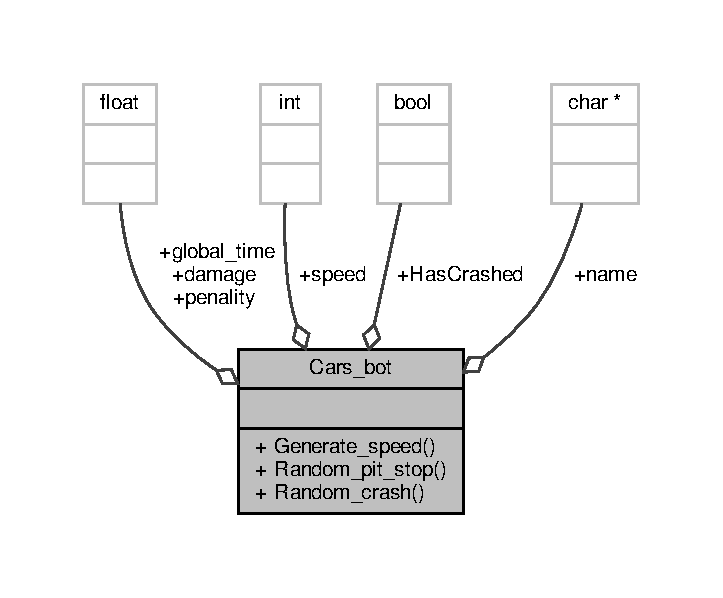
\includegraphics[width=347pt]{class_cars__bot__coll__graph}
\end{center}
\end{figure}
\subsection*{Public Member Functions}
\begin{DoxyCompactItemize}
\item 
void \hyperlink{class_cars__bot_a79d7a174260eb5c633b3067dbdef04e5}{Generate\+\_\+speed} ()
\item 
void \hyperlink{class_cars__bot_a16a23b35ae128f5b905c0d95f56f916e}{Random\+\_\+pit\+\_\+stop} ()
\item 
void \hyperlink{class_cars__bot_ab7d72e0c79e5efd16a0242c950e0dbf8}{Random\+\_\+crash} ()
\end{DoxyCompactItemize}
\subsection*{Public Attributes}
\begin{DoxyCompactItemize}
\item 
int \hyperlink{class_cars__bot_aa1c5f72aa6b013435bab77408fd56388}{speed} = 0
\begin{DoxyCompactList}\small\item\em Average speed last lap. \end{DoxyCompactList}\item 
float \hyperlink{class_cars__bot_a358a371bdfed0782a07a958b7868b0e2}{damage} = 0.\+0
\begin{DoxyCompactList}\small\item\em Damage due to collision. \end{DoxyCompactList}\item 
float \hyperlink{class_cars__bot_a61c7db007ee9ea521ba5369ab7d76e1e}{penality} = 0
\begin{DoxyCompactList}\small\item\em Time penality is the time the car is at pit stop. \end{DoxyCompactList}\item 
float \hyperlink{class_cars__bot_ad58234570f5051e4a607da5351cf1b78}{global\+\_\+time} = 0
\begin{DoxyCompactList}\small\item\em Global race time of the car ~\newline
 Can be set at 40404 aka \char`\"{}\+Crash time\char`\"{} to identify that a car has crash in the leaderboard. \end{DoxyCompactList}\item 
char $\ast$ \hyperlink{class_cars__bot_af68fbb76d9a894060bc33b9837d50796}{name} = \char`\"{}undefined\char`\"{}
\begin{DoxyCompactList}\small\item\em Car\textquotesingle{}s name. \end{DoxyCompactList}\item 
bool \hyperlink{class_cars__bot_a727a25c57ca410c714bf66edf809b469}{Has\+Crashed} = false
\begin{DoxyCompactList}\small\item\em If has crashed (Due to collision or not) \end{DoxyCompactList}\end{DoxyCompactItemize}


\subsection{Member Function Documentation}
\mbox{\Hypertarget{class_cars__bot_a79d7a174260eb5c633b3067dbdef04e5}\label{class_cars__bot_a79d7a174260eb5c633b3067dbdef04e5}} 
\index{Cars\+\_\+bot@{Cars\+\_\+bot}!Generate\+\_\+speed@{Generate\+\_\+speed}}
\index{Generate\+\_\+speed@{Generate\+\_\+speed}!Cars\+\_\+bot@{Cars\+\_\+bot}}
\subsubsection{\texorpdfstring{Generate\+\_\+speed()}{Generate\_speed()}}
{\footnotesize\ttfamily void Cars\+\_\+bot\+::\+Generate\+\_\+speed (\begin{DoxyParamCaption}{ }\end{DoxyParamCaption})}

Randomly generate car average speed during a lap

Minimum average speed = 200 km/h Maximum average speed = 323 km/h \mbox{\Hypertarget{class_cars__bot_ab7d72e0c79e5efd16a0242c950e0dbf8}\label{class_cars__bot_ab7d72e0c79e5efd16a0242c950e0dbf8}} 
\index{Cars\+\_\+bot@{Cars\+\_\+bot}!Random\+\_\+crash@{Random\+\_\+crash}}
\index{Random\+\_\+crash@{Random\+\_\+crash}!Cars\+\_\+bot@{Cars\+\_\+bot}}
\subsubsection{\texorpdfstring{Random\+\_\+crash()}{Random\_crash()}}
{\footnotesize\ttfamily void Cars\+\_\+bot\+::\+Random\+\_\+crash (\begin{DoxyParamCaption}{ }\end{DoxyParamCaption})}

Randomly generate a car crash

1 in 1000 chance that the bot will crash

set global time to \char`\"{}\+Crash Time\char`\"{} \mbox{\Hypertarget{class_cars__bot_a16a23b35ae128f5b905c0d95f56f916e}\label{class_cars__bot_a16a23b35ae128f5b905c0d95f56f916e}} 
\index{Cars\+\_\+bot@{Cars\+\_\+bot}!Random\+\_\+pit\+\_\+stop@{Random\+\_\+pit\+\_\+stop}}
\index{Random\+\_\+pit\+\_\+stop@{Random\+\_\+pit\+\_\+stop}!Cars\+\_\+bot@{Cars\+\_\+bot}}
\subsubsection{\texorpdfstring{Random\+\_\+pit\+\_\+stop()}{Random\_pit\_stop()}}
{\footnotesize\ttfamily void Cars\+\_\+bot\+::\+Random\+\_\+pit\+\_\+stop (\begin{DoxyParamCaption}{ }\end{DoxyParamCaption})}

Randomly generate a pit stop

Needed for balancing reasons

10 \% chance that the bot will stop

add a random penality between 0 and 20 sec 

\subsection{Member Data Documentation}
\mbox{\Hypertarget{class_cars__bot_a358a371bdfed0782a07a958b7868b0e2}\label{class_cars__bot_a358a371bdfed0782a07a958b7868b0e2}} 
\index{Cars\+\_\+bot@{Cars\+\_\+bot}!damage@{damage}}
\index{damage@{damage}!Cars\+\_\+bot@{Cars\+\_\+bot}}
\subsubsection{\texorpdfstring{damage}{damage}}
{\footnotesize\ttfamily float Cars\+\_\+bot\+::damage = 0.\+0}



Damage due to collision. 

\mbox{\Hypertarget{class_cars__bot_ad58234570f5051e4a607da5351cf1b78}\label{class_cars__bot_ad58234570f5051e4a607da5351cf1b78}} 
\index{Cars\+\_\+bot@{Cars\+\_\+bot}!global\+\_\+time@{global\+\_\+time}}
\index{global\+\_\+time@{global\+\_\+time}!Cars\+\_\+bot@{Cars\+\_\+bot}}
\subsubsection{\texorpdfstring{global\+\_\+time}{global\_time}}
{\footnotesize\ttfamily float Cars\+\_\+bot\+::global\+\_\+time = 0}



Global race time of the car ~\newline
 Can be set at 40404 aka \char`\"{}\+Crash time\char`\"{} to identify that a car has crash in the leaderboard. 

\mbox{\Hypertarget{class_cars__bot_a727a25c57ca410c714bf66edf809b469}\label{class_cars__bot_a727a25c57ca410c714bf66edf809b469}} 
\index{Cars\+\_\+bot@{Cars\+\_\+bot}!Has\+Crashed@{Has\+Crashed}}
\index{Has\+Crashed@{Has\+Crashed}!Cars\+\_\+bot@{Cars\+\_\+bot}}
\subsubsection{\texorpdfstring{Has\+Crashed}{HasCrashed}}
{\footnotesize\ttfamily bool Cars\+\_\+bot\+::\+Has\+Crashed = false}



If has crashed (Due to collision or not) 

\mbox{\Hypertarget{class_cars__bot_af68fbb76d9a894060bc33b9837d50796}\label{class_cars__bot_af68fbb76d9a894060bc33b9837d50796}} 
\index{Cars\+\_\+bot@{Cars\+\_\+bot}!name@{name}}
\index{name@{name}!Cars\+\_\+bot@{Cars\+\_\+bot}}
\subsubsection{\texorpdfstring{name}{name}}
{\footnotesize\ttfamily char$\ast$ Cars\+\_\+bot\+::name = \char`\"{}undefined\char`\"{}}



Car\textquotesingle{}s name. 

\mbox{\Hypertarget{class_cars__bot_a61c7db007ee9ea521ba5369ab7d76e1e}\label{class_cars__bot_a61c7db007ee9ea521ba5369ab7d76e1e}} 
\index{Cars\+\_\+bot@{Cars\+\_\+bot}!penality@{penality}}
\index{penality@{penality}!Cars\+\_\+bot@{Cars\+\_\+bot}}
\subsubsection{\texorpdfstring{penality}{penality}}
{\footnotesize\ttfamily float Cars\+\_\+bot\+::penality = 0}



Time penality is the time the car is at pit stop. 

\mbox{\Hypertarget{class_cars__bot_aa1c5f72aa6b013435bab77408fd56388}\label{class_cars__bot_aa1c5f72aa6b013435bab77408fd56388}} 
\index{Cars\+\_\+bot@{Cars\+\_\+bot}!speed@{speed}}
\index{speed@{speed}!Cars\+\_\+bot@{Cars\+\_\+bot}}
\subsubsection{\texorpdfstring{speed}{speed}}
{\footnotesize\ttfamily int Cars\+\_\+bot\+::speed = 0}



Average speed last lap. 



The documentation for this class was generated from the following files\+:\begin{DoxyCompactItemize}
\item 
Classes/\hyperlink{_cars__bot_8h}{Cars\+\_\+bot.\+h}\item 
Classes/\hyperlink{_cars__bot_8cpp}{Cars\+\_\+bot.\+cpp}\end{DoxyCompactItemize}

\hypertarget{class_circuit}{}\section{Circuit Class Reference}
\label{class_circuit}\index{Circuit@{Circuit}}


{\ttfamily \#include $<$Circuit.\+h$>$}



Collaboration diagram for Circuit\+:
\nopagebreak
\begin{figure}[H]
\begin{center}
\leavevmode
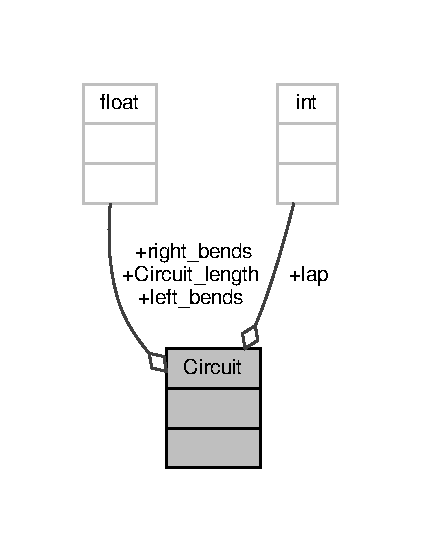
\includegraphics[width=202pt]{class_circuit__coll__graph}
\end{center}
\end{figure}
\subsection*{Public Attributes}
\begin{DoxyCompactItemize}
\item 
int \hyperlink{class_circuit_a6bdf0f1b4883feb6d010c104c336c5ef}{lap} = 50
\begin{DoxyCompactList}\small\item\em Number of laps in the race. \end{DoxyCompactList}\item 
float \hyperlink{class_circuit_ad4816f23069209f47517ea3566e43e09}{Circuit\+\_\+length} = 5371.\+0
\begin{DoxyCompactList}\small\item\em \hyperlink{class_circuit}{Circuit} length in meter. \end{DoxyCompactList}\item 
float \hyperlink{class_circuit_a3b64033e71ea613856d1054d741f0dea}{right\+\_\+bends} = 4.\+0
\begin{DoxyCompactList}\small\item\em Number of right bends in the circuit. \end{DoxyCompactList}\item 
float \hyperlink{class_circuit_ac5eee1d1d6ea557388881e15c311e181}{left\+\_\+bends} = 5.\+0
\begin{DoxyCompactList}\small\item\em Number of left bends in the circuit. \end{DoxyCompactList}\end{DoxyCompactItemize}


\subsection{Member Data Documentation}
\mbox{\Hypertarget{class_circuit_ad4816f23069209f47517ea3566e43e09}\label{class_circuit_ad4816f23069209f47517ea3566e43e09}} 
\index{Circuit@{Circuit}!Circuit\+\_\+length@{Circuit\+\_\+length}}
\index{Circuit\+\_\+length@{Circuit\+\_\+length}!Circuit@{Circuit}}
\subsubsection{\texorpdfstring{Circuit\+\_\+length}{Circuit\_length}}
{\footnotesize\ttfamily float Circuit\+::\+Circuit\+\_\+length = 5371.\+0}



\hyperlink{class_circuit}{Circuit} length in meter. 

\mbox{\Hypertarget{class_circuit_a6bdf0f1b4883feb6d010c104c336c5ef}\label{class_circuit_a6bdf0f1b4883feb6d010c104c336c5ef}} 
\index{Circuit@{Circuit}!lap@{lap}}
\index{lap@{lap}!Circuit@{Circuit}}
\subsubsection{\texorpdfstring{lap}{lap}}
{\footnotesize\ttfamily int Circuit\+::lap = 50}



Number of laps in the race. 

\mbox{\Hypertarget{class_circuit_ac5eee1d1d6ea557388881e15c311e181}\label{class_circuit_ac5eee1d1d6ea557388881e15c311e181}} 
\index{Circuit@{Circuit}!left\+\_\+bends@{left\+\_\+bends}}
\index{left\+\_\+bends@{left\+\_\+bends}!Circuit@{Circuit}}
\subsubsection{\texorpdfstring{left\+\_\+bends}{left\_bends}}
{\footnotesize\ttfamily float Circuit\+::left\+\_\+bends = 5.\+0}



Number of left bends in the circuit. 

\mbox{\Hypertarget{class_circuit_a3b64033e71ea613856d1054d741f0dea}\label{class_circuit_a3b64033e71ea613856d1054d741f0dea}} 
\index{Circuit@{Circuit}!right\+\_\+bends@{right\+\_\+bends}}
\index{right\+\_\+bends@{right\+\_\+bends}!Circuit@{Circuit}}
\subsubsection{\texorpdfstring{right\+\_\+bends}{right\_bends}}
{\footnotesize\ttfamily float Circuit\+::right\+\_\+bends = 4.\+0}



Number of right bends in the circuit. 



The documentation for this class was generated from the following file\+:\begin{DoxyCompactItemize}
\item 
Classes/\hyperlink{_circuit_8h}{Circuit.\+h}\end{DoxyCompactItemize}

\hypertarget{class_race}{}\section{Race Class Reference}
\label{class_race}\index{Race@{Race}}


{\ttfamily \#include $<$Race.\+h$>$}



Collaboration diagram for Race\+:
\nopagebreak
\begin{figure}[H]
\begin{center}
\leavevmode
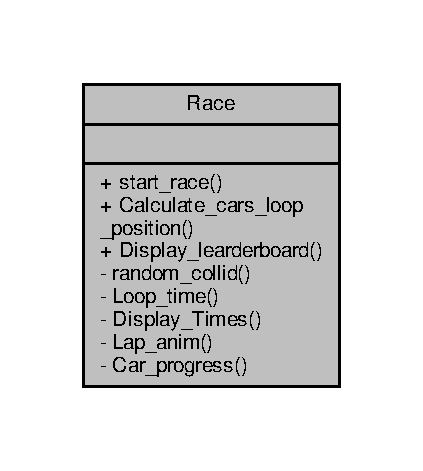
\includegraphics[width=203pt]{class_race__coll__graph}
\end{center}
\end{figure}
\subsection*{Static Public Member Functions}
\begin{DoxyCompactItemize}
\item 
static void \hyperlink{class_race_a4689c08e7e82f81bbd5f2173cf80f2e2}{start\+\_\+race} ()
\item 
static void \hyperlink{class_race_a1f46c8f5eb505d88620264f0d8f6b22c}{Calculate\+\_\+cars\+\_\+loop\+\_\+position} ()
\item 
static void \hyperlink{class_race_a60746a5c9eb52b2977a3c601a3c176d7}{Display\+\_\+learderboard} ()
\end{DoxyCompactItemize}
\subsection*{Static Private Member Functions}
\begin{DoxyCompactItemize}
\item 
static void \hyperlink{class_race_a39c85f002d23e5f69eb41130d56d8a0f}{random\+\_\+collid} ()
\item 
static float \hyperlink{class_race_a75246185d954052dd7a0d19b4fdda1a4}{Loop\+\_\+time} (float Circuit\+\_\+length, float Car\+\_\+speed, float penality)
\item 
static void \hyperlink{class_race_a45900e00f7218173658537ac6a2cda86}{Display\+\_\+\+Times} ()
\item 
static void \hyperlink{class_race_ac1ba3c7832ec62812a2fdd21f7fbd46c}{Lap\+\_\+anim} ()
\item 
static char $\ast$ \hyperlink{class_race_a4ce05f7770cfe6fe888b0a3bbdb87b83}{Car\+\_\+progress} (float elapsed\+\_\+time, float Total\+\_\+time)
\end{DoxyCompactItemize}


\subsection{Member Function Documentation}
\mbox{\Hypertarget{class_race_a1f46c8f5eb505d88620264f0d8f6b22c}\label{class_race_a1f46c8f5eb505d88620264f0d8f6b22c}} 
\index{Race@{Race}!Calculate\+\_\+cars\+\_\+loop\+\_\+position@{Calculate\+\_\+cars\+\_\+loop\+\_\+position}}
\index{Calculate\+\_\+cars\+\_\+loop\+\_\+position@{Calculate\+\_\+cars\+\_\+loop\+\_\+position}!Race@{Race}}
\subsubsection{\texorpdfstring{Calculate\+\_\+cars\+\_\+loop\+\_\+position()}{Calculate\_cars\_loop\_position()}}
{\footnotesize\ttfamily void Race\+::\+Calculate\+\_\+cars\+\_\+loop\+\_\+position (\begin{DoxyParamCaption}{ }\end{DoxyParamCaption})\hspace{0.3cm}{\ttfamily [static]}}

Calculate the position of all the cars in the race \mbox{\Hypertarget{class_race_a4ce05f7770cfe6fe888b0a3bbdb87b83}\label{class_race_a4ce05f7770cfe6fe888b0a3bbdb87b83}} 
\index{Race@{Race}!Car\+\_\+progress@{Car\+\_\+progress}}
\index{Car\+\_\+progress@{Car\+\_\+progress}!Race@{Race}}
\subsubsection{\texorpdfstring{Car\+\_\+progress()}{Car\_progress()}}
{\footnotesize\ttfamily char $\ast$ Race\+::\+Car\+\_\+progress (\begin{DoxyParamCaption}\item[{float}]{elapsed\+\_\+time,  }\item[{float}]{Total\+\_\+time }\end{DoxyParamCaption})\hspace{0.3cm}{\ttfamily [static]}, {\ttfamily [private]}}

Our anim is a progress bar that has 10 progress point

when a car has done 1/10 of the lap it add an \char`\"{}\#\char`\"{} ~\newline
 exemple \+: \mbox{[}\#\#\+\_\+\+\_\+\+\_\+\+\_\+\+\_\+\+\_\+\+\_\+\mbox{]} when the car has done more than 2/10 of the lap ( \char`\"{}\+\_\+\char`\"{} are space ) \mbox{\Hypertarget{class_race_a60746a5c9eb52b2977a3c601a3c176d7}\label{class_race_a60746a5c9eb52b2977a3c601a3c176d7}} 
\index{Race@{Race}!Display\+\_\+learderboard@{Display\+\_\+learderboard}}
\index{Display\+\_\+learderboard@{Display\+\_\+learderboard}!Race@{Race}}
\subsubsection{\texorpdfstring{Display\+\_\+learderboard()}{Display\_learderboard()}}
{\footnotesize\ttfamily void Race\+::\+Display\+\_\+learderboard (\begin{DoxyParamCaption}{ }\end{DoxyParamCaption})\hspace{0.3cm}{\ttfamily [static]}}

Display a ranking of all the cars in the race \mbox{\Hypertarget{class_race_a45900e00f7218173658537ac6a2cda86}\label{class_race_a45900e00f7218173658537ac6a2cda86}} 
\index{Race@{Race}!Display\+\_\+\+Times@{Display\+\_\+\+Times}}
\index{Display\+\_\+\+Times@{Display\+\_\+\+Times}!Race@{Race}}
\subsubsection{\texorpdfstring{Display\+\_\+\+Times()}{Display\_Times()}}
{\footnotesize\ttfamily void Race\+::\+Display\+\_\+\+Times (\begin{DoxyParamCaption}{ }\end{DoxyParamCaption})\hspace{0.3cm}{\ttfamily [static]}, {\ttfamily [private]}}

Display the time of the player\textquotesingle{}s cars and their position in the race \mbox{\Hypertarget{class_race_ac1ba3c7832ec62812a2fdd21f7fbd46c}\label{class_race_ac1ba3c7832ec62812a2fdd21f7fbd46c}} 
\index{Race@{Race}!Lap\+\_\+anim@{Lap\+\_\+anim}}
\index{Lap\+\_\+anim@{Lap\+\_\+anim}!Race@{Race}}
\subsubsection{\texorpdfstring{Lap\+\_\+anim()}{Lap\_anim()}}
{\footnotesize\ttfamily void Race\+::\+Lap\+\_\+anim (\begin{DoxyParamCaption}{ }\end{DoxyParamCaption})\hspace{0.3cm}{\ttfamily [static]}, {\ttfamily [private]}}

Display an animation of the progress of the player\textquotesingle{}s cars in the lap \mbox{\Hypertarget{class_race_a75246185d954052dd7a0d19b4fdda1a4}\label{class_race_a75246185d954052dd7a0d19b4fdda1a4}} 
\index{Race@{Race}!Loop\+\_\+time@{Loop\+\_\+time}}
\index{Loop\+\_\+time@{Loop\+\_\+time}!Race@{Race}}
\subsubsection{\texorpdfstring{Loop\+\_\+time()}{Loop\_time()}}
{\footnotesize\ttfamily float Race\+::\+Loop\+\_\+time (\begin{DoxyParamCaption}\item[{float}]{Circuit\+\_\+length,  }\item[{float}]{Car\+\_\+speed,  }\item[{float}]{penality }\end{DoxyParamCaption})\hspace{0.3cm}{\ttfamily [static]}, {\ttfamily [private]}}

calculates the time it took a car to complete the lap.

loop time equal travel time + time penality \mbox{\Hypertarget{class_race_a39c85f002d23e5f69eb41130d56d8a0f}\label{class_race_a39c85f002d23e5f69eb41130d56d8a0f}} 
\index{Race@{Race}!random\+\_\+collid@{random\+\_\+collid}}
\index{random\+\_\+collid@{random\+\_\+collid}!Race@{Race}}
\subsubsection{\texorpdfstring{random\+\_\+collid()}{random\_collid()}}
{\footnotesize\ttfamily void Race\+::random\+\_\+collid (\begin{DoxyParamCaption}{ }\end{DoxyParamCaption})\hspace{0.3cm}{\ttfamily [static]}, {\ttfamily [private]}}

Generate random collision between cars

1 in 50 chance that there will be a collision this lap

If the impact is too violent, colliding vehicles may crash.

Can have multiple collision \mbox{\Hypertarget{class_race_a4689c08e7e82f81bbd5f2173cf80f2e2}\label{class_race_a4689c08e7e82f81bbd5f2173cf80f2e2}} 
\index{Race@{Race}!start\+\_\+race@{start\+\_\+race}}
\index{start\+\_\+race@{start\+\_\+race}!Race@{Race}}
\subsubsection{\texorpdfstring{start\+\_\+race()}{start\_race()}}
{\footnotesize\ttfamily void Race\+::start\+\_\+race (\begin{DoxyParamCaption}{ }\end{DoxyParamCaption})\hspace{0.3cm}{\ttfamily [static]}}

Start the race 

The documentation for this class was generated from the following files\+:\begin{DoxyCompactItemize}
\item 
Classes/\hyperlink{_race_8h}{Race.\+h}\item 
Classes/\hyperlink{_race_8cpp}{Race.\+cpp}\end{DoxyCompactItemize}

\hypertarget{classutils}{}\section{utils Class Reference}
\label{classutils}\index{utils@{utils}}


{\ttfamily \#include $<$utils.\+h$>$}



Collaboration diagram for utils\+:
\nopagebreak
\begin{figure}[H]
\begin{center}
\leavevmode
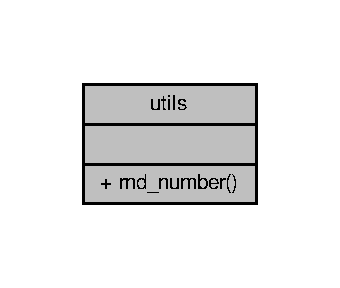
\includegraphics[width=163pt]{classutils__coll__graph}
\end{center}
\end{figure}
\subsection*{Static Public Member Functions}
\begin{DoxyCompactItemize}
\item 
static int \hyperlink{classutils_a4b8ed2e14db429698b2e2694c80bfb04}{rnd\+\_\+number} (float min, float max)
\end{DoxyCompactItemize}


\subsection{Member Function Documentation}
\mbox{\Hypertarget{classutils_a4b8ed2e14db429698b2e2694c80bfb04}\label{classutils_a4b8ed2e14db429698b2e2694c80bfb04}} 
\index{utils@{utils}!rnd\+\_\+number@{rnd\+\_\+number}}
\index{rnd\+\_\+number@{rnd\+\_\+number}!utils@{utils}}
\subsubsection{\texorpdfstring{rnd\+\_\+number()}{rnd\_number()}}
{\footnotesize\ttfamily int utils\+::rnd\+\_\+number (\begin{DoxyParamCaption}\item[{float}]{min,  }\item[{float}]{max }\end{DoxyParamCaption})\hspace{0.3cm}{\ttfamily [static]}}

Generate a random floating number between min and max

use Mersenne Twister 19937 generator

A Mersenne Twister pseudo-\/random generator of 32-\/bit numbers with a state size of 19937 bits. 

The documentation for this class was generated from the following files\+:\begin{DoxyCompactItemize}
\item 
Classes/\hyperlink{utils_8h}{utils.\+h}\item 
Classes/\hyperlink{utils_8cpp}{utils.\+cpp}\end{DoxyCompactItemize}

\chapter{File Documentation}
\hypertarget{_cars_8cpp}{}\section{Classes/\+Cars.cpp File Reference}
\label{_cars_8cpp}\index{Classes/\+Cars.\+cpp@{Classes/\+Cars.\+cpp}}
{\ttfamily \#include $<$iostream$>$}\newline
{\ttfamily \#include \char`\"{}Cars.\+h\char`\"{}}\newline
{\ttfamily \#include \char`\"{}utils.\+h\char`\"{}}\newline
Include dependency graph for Cars.\+cpp\+:
\nopagebreak
\begin{figure}[H]
\begin{center}
\leavevmode
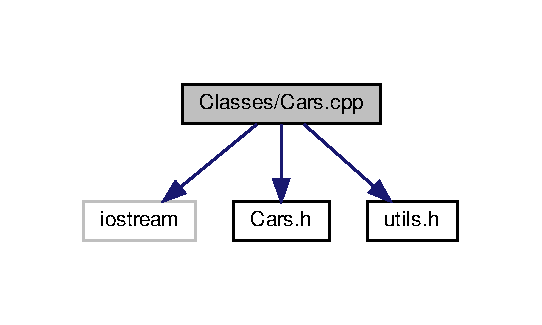
\includegraphics[width=260pt]{_cars_8cpp__incl}
\end{center}
\end{figure}

\hypertarget{_cars_8h}{}\section{Classes/\+Cars.h File Reference}
\label{_cars_8h}\index{Classes/\+Cars.\+h@{Classes/\+Cars.\+h}}
This graph shows which files directly or indirectly include this file\+:
\nopagebreak
\begin{figure}[H]
\begin{center}
\leavevmode
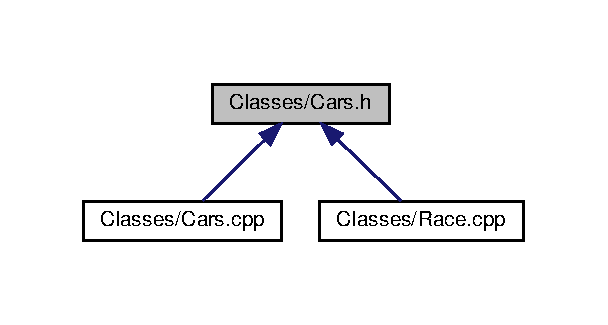
\includegraphics[width=292pt]{_cars_8h__dep__incl}
\end{center}
\end{figure}
\subsection*{Classes}
\begin{DoxyCompactItemize}
\item 
class \hyperlink{class_cars}{Cars}
\end{DoxyCompactItemize}

\hypertarget{_cars__bot_8cpp}{}\section{Classes/\+Cars\+\_\+bot.cpp File Reference}
\label{_cars__bot_8cpp}\index{Classes/\+Cars\+\_\+bot.\+cpp@{Classes/\+Cars\+\_\+bot.\+cpp}}
{\ttfamily \#include \char`\"{}Cars\+\_\+bot.\+h\char`\"{}}\newline
{\ttfamily \#include \char`\"{}utils.\+h\char`\"{}}\newline
Include dependency graph for Cars\+\_\+bot.\+cpp\+:
\nopagebreak
\begin{figure}[H]
\begin{center}
\leavevmode
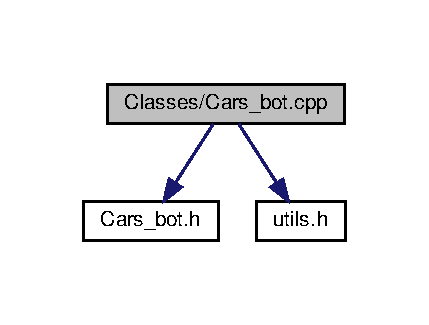
\includegraphics[width=206pt]{_cars__bot_8cpp__incl}
\end{center}
\end{figure}

\hypertarget{_cars__bot_8h}{}\section{Classes/\+Cars\+\_\+bot.h File Reference}
\label{_cars__bot_8h}\index{Classes/\+Cars\+\_\+bot.\+h@{Classes/\+Cars\+\_\+bot.\+h}}
This graph shows which files directly or indirectly include this file\+:
\nopagebreak
\begin{figure}[H]
\begin{center}
\leavevmode
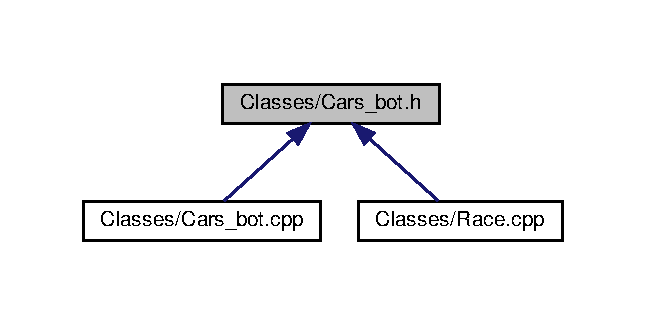
\includegraphics[width=310pt]{_cars__bot_8h__dep__incl}
\end{center}
\end{figure}
\subsection*{Classes}
\begin{DoxyCompactItemize}
\item 
class \hyperlink{class_cars__bot}{Cars\+\_\+bot}
\end{DoxyCompactItemize}

\hypertarget{_circuit_8cpp}{}\section{Classes/\+Circuit.cpp File Reference}
\label{_circuit_8cpp}\index{Classes/\+Circuit.\+cpp@{Classes/\+Circuit.\+cpp}}
{\ttfamily \#include \char`\"{}Circuit.\+h\char`\"{}}\newline
Include dependency graph for Circuit.\+cpp\+:
\nopagebreak
\begin{figure}[H]
\begin{center}
\leavevmode
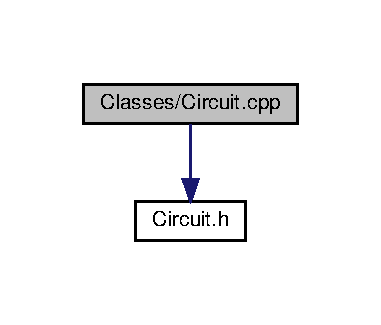
\includegraphics[width=183pt]{_circuit_8cpp__incl}
\end{center}
\end{figure}

\hypertarget{_circuit_8h}{}\section{Classes/\+Circuit.h File Reference}
\label{_circuit_8h}\index{Classes/\+Circuit.\+h@{Classes/\+Circuit.\+h}}
This graph shows which files directly or indirectly include this file\+:
\nopagebreak
\begin{figure}[H]
\begin{center}
\leavevmode
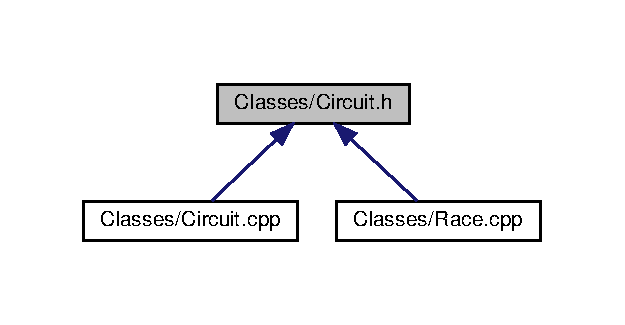
\includegraphics[width=300pt]{_circuit_8h__dep__incl}
\end{center}
\end{figure}
\subsection*{Classes}
\begin{DoxyCompactItemize}
\item 
class \hyperlink{class_circuit}{Circuit}
\end{DoxyCompactItemize}

\hypertarget{_race_8cpp}{}\section{Classes/\+Race.cpp File Reference}
\label{_race_8cpp}\index{Classes/\+Race.\+cpp@{Classes/\+Race.\+cpp}}
{\ttfamily \#include $<$iostream$>$}\newline
{\ttfamily \#include $<$cstring$>$}\newline
{\ttfamily \#include \char`\"{}utils.\+h\char`\"{}}\newline
{\ttfamily \#include \char`\"{}Race.\+h\char`\"{}}\newline
{\ttfamily \#include \char`\"{}Cars.\+h\char`\"{}}\newline
{\ttfamily \#include \char`\"{}Circuit.\+h\char`\"{}}\newline
{\ttfamily \#include \char`\"{}Cars\+\_\+bot.\+h\char`\"{}}\newline
{\ttfamily \#include $<$chrono$>$}\newline
{\ttfamily \#include $<$thread$>$}\newline
{\ttfamily \#include $<$algorithm$>$}\newline
Include dependency graph for Race.\+cpp\+:
\nopagebreak
\begin{figure}[H]
\begin{center}
\leavevmode
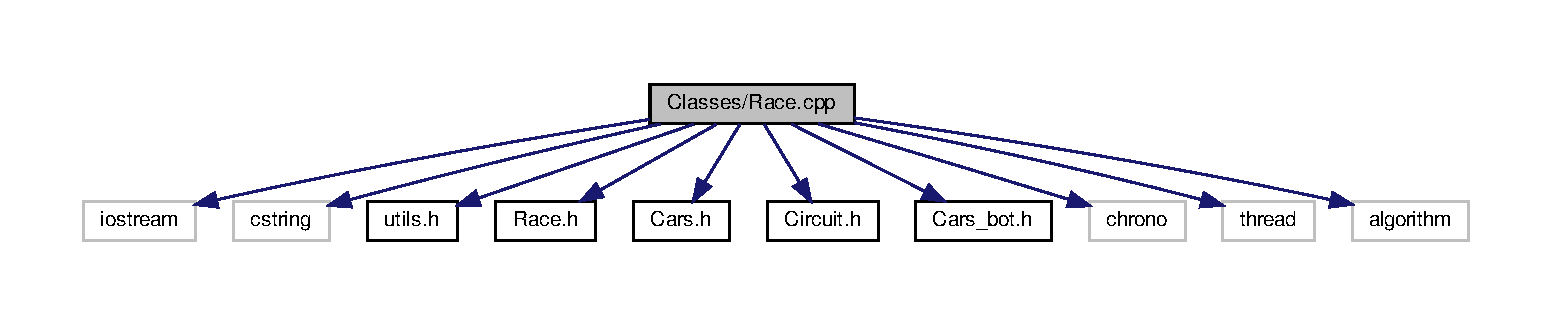
\includegraphics[width=350pt]{_race_8cpp__incl}
\end{center}
\end{figure}
\subsection*{Variables}
\begin{DoxyCompactItemize}
\item 
char $\ast$ \hyperlink{_race_8cpp_a59e3e74358e8dff27cd79c4952bbc672}{bot\+\_\+namelist} \mbox{[}21\mbox{]}
\item 
\hyperlink{class_circuit}{Circuit} \hyperlink{_race_8cpp_a9c34580abc41088874c5da33bb22ef80}{Paul\+\_\+\+Ricard}
\begin{DoxyCompactList}\small\item\em location \char`\"{}\+Le Castellet\char`\"{},France \end{DoxyCompactList}\item 
\hyperlink{class_cars}{Cars} \hyperlink{_race_8cpp_a4f5c1b540e06419c45da2d1e21247cd4}{Car1}
\item 
\hyperlink{class_cars}{Cars} \hyperlink{_race_8cpp_a549ada0a437dbbc0955b6a8d726ba5df}{Car2}
\item 
const int \hyperlink{_race_8cpp_a7818c1dd81ef6d51a51ca6bf590cc2f8}{N\+B\+\_\+\+B\+OT} = 20
\begin{DoxyCompactList}\small\item\em define the number of bots during the race \end{DoxyCompactList}\item 
\hyperlink{class_cars__bot}{Cars\+\_\+bot} $\ast$ \hyperlink{_race_8cpp_adf2ed4f50293bd894d5b3b8a810393f7}{bot} = new \hyperlink{class_cars__bot}{Cars\+\_\+bot}\mbox{[}\hyperlink{_race_8cpp_a7818c1dd81ef6d51a51ca6bf590cc2f8}{N\+B\+\_\+\+B\+OT}\mbox{]}
\end{DoxyCompactItemize}


\subsection{Variable Documentation}
\mbox{\Hypertarget{_race_8cpp_adf2ed4f50293bd894d5b3b8a810393f7}\label{_race_8cpp_adf2ed4f50293bd894d5b3b8a810393f7}} 
\index{Race.\+cpp@{Race.\+cpp}!bot@{bot}}
\index{bot@{bot}!Race.\+cpp@{Race.\+cpp}}
\subsubsection{\texorpdfstring{bot}{bot}}
{\footnotesize\ttfamily \hyperlink{class_cars__bot}{Cars\+\_\+bot}$\ast$ bot = new \hyperlink{class_cars__bot}{Cars\+\_\+bot}\mbox{[}\hyperlink{_race_8cpp_a7818c1dd81ef6d51a51ca6bf590cc2f8}{N\+B\+\_\+\+B\+OT}\mbox{]}}

\mbox{\Hypertarget{_race_8cpp_a59e3e74358e8dff27cd79c4952bbc672}\label{_race_8cpp_a59e3e74358e8dff27cd79c4952bbc672}} 
\index{Race.\+cpp@{Race.\+cpp}!bot\+\_\+namelist@{bot\+\_\+namelist}}
\index{bot\+\_\+namelist@{bot\+\_\+namelist}!Race.\+cpp@{Race.\+cpp}}
\subsubsection{\texorpdfstring{bot\+\_\+namelist}{bot\_namelist}}
{\footnotesize\ttfamily char$\ast$ bot\+\_\+namelist\mbox{[}21\mbox{]}}

{\bfseries Initial value\+:}
\begin{DoxyCode}
= \{\textcolor{stringliteral}{"Bertand"}, \textcolor{stringliteral}{"Bernie"}, \textcolor{stringliteral}{"Olive"}, \textcolor{stringliteral}{"Paul"}, \textcolor{stringliteral}{"Jacob"}, \textcolor{stringliteral}{"Maxon"}, \textcolor{stringliteral}{"Laurent"},
                          \textcolor{stringliteral}{"Aurelie"}, \textcolor{stringliteral}{"Quentin"}, \textcolor{stringliteral}{"Alban"}, \textcolor{stringliteral}{"Judicael"}, \textcolor{stringliteral}{"Alick"}, \textcolor{stringliteral}{"Alcapone"},
                          \textcolor{stringliteral}{"Estelle"}, \textcolor{stringliteral}{"Cyril"}, \textcolor{stringliteral}{"Emma"}, \textcolor{stringliteral}{"Mohamed"}, \textcolor{stringliteral}{"Barack"}, \textcolor{stringliteral}{"Clara"}, \textcolor{stringliteral}{"Lancelot"},
                          \textcolor{stringliteral}{"Pierre"}\}
\end{DoxyCode}
\mbox{\Hypertarget{_race_8cpp_a4f5c1b540e06419c45da2d1e21247cd4}\label{_race_8cpp_a4f5c1b540e06419c45da2d1e21247cd4}} 
\index{Race.\+cpp@{Race.\+cpp}!Car1@{Car1}}
\index{Car1@{Car1}!Race.\+cpp@{Race.\+cpp}}
\subsubsection{\texorpdfstring{Car1}{Car1}}
{\footnotesize\ttfamily \hyperlink{class_cars}{Cars} Car1}

\mbox{\Hypertarget{_race_8cpp_a549ada0a437dbbc0955b6a8d726ba5df}\label{_race_8cpp_a549ada0a437dbbc0955b6a8d726ba5df}} 
\index{Race.\+cpp@{Race.\+cpp}!Car2@{Car2}}
\index{Car2@{Car2}!Race.\+cpp@{Race.\+cpp}}
\subsubsection{\texorpdfstring{Car2}{Car2}}
{\footnotesize\ttfamily \hyperlink{class_cars}{Cars} Car2}

\mbox{\Hypertarget{_race_8cpp_a7818c1dd81ef6d51a51ca6bf590cc2f8}\label{_race_8cpp_a7818c1dd81ef6d51a51ca6bf590cc2f8}} 
\index{Race.\+cpp@{Race.\+cpp}!N\+B\+\_\+\+B\+OT@{N\+B\+\_\+\+B\+OT}}
\index{N\+B\+\_\+\+B\+OT@{N\+B\+\_\+\+B\+OT}!Race.\+cpp@{Race.\+cpp}}
\subsubsection{\texorpdfstring{N\+B\+\_\+\+B\+OT}{NB\_BOT}}
{\footnotesize\ttfamily const int N\+B\+\_\+\+B\+OT = 20}



define the number of bots during the race 

\mbox{\Hypertarget{_race_8cpp_a9c34580abc41088874c5da33bb22ef80}\label{_race_8cpp_a9c34580abc41088874c5da33bb22ef80}} 
\index{Race.\+cpp@{Race.\+cpp}!Paul\+\_\+\+Ricard@{Paul\+\_\+\+Ricard}}
\index{Paul\+\_\+\+Ricard@{Paul\+\_\+\+Ricard}!Race.\+cpp@{Race.\+cpp}}
\subsubsection{\texorpdfstring{Paul\+\_\+\+Ricard}{Paul\_Ricard}}
{\footnotesize\ttfamily \hyperlink{class_circuit}{Circuit} Paul\+\_\+\+Ricard}



location \char`\"{}\+Le Castellet\char`\"{},France 


\hypertarget{_race_8h}{}\section{Classes/\+Race.h File Reference}
\label{_race_8h}\index{Classes/\+Race.\+h@{Classes/\+Race.\+h}}
This graph shows which files directly or indirectly include this file\+:
\nopagebreak
\begin{figure}[H]
\begin{center}
\leavevmode
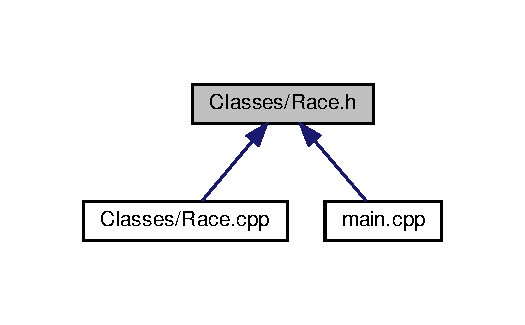
\includegraphics[width=252pt]{_race_8h__dep__incl}
\end{center}
\end{figure}
\subsection*{Classes}
\begin{DoxyCompactItemize}
\item 
class \hyperlink{class_race}{Race}
\end{DoxyCompactItemize}

\hypertarget{utils_8cpp}{}\section{Classes/utils.cpp File Reference}
\label{utils_8cpp}\index{Classes/utils.\+cpp@{Classes/utils.\+cpp}}
{\ttfamily \#include $<$random$>$}\newline
{\ttfamily \#include \char`\"{}utils.\+h\char`\"{}}\newline
Include dependency graph for utils.\+cpp\+:
\nopagebreak
\begin{figure}[H]
\begin{center}
\leavevmode
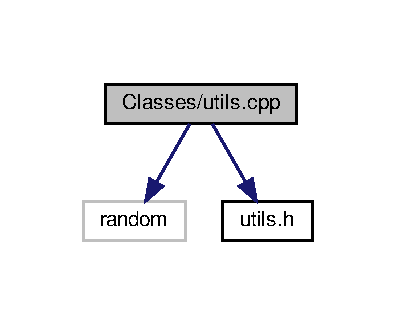
\includegraphics[width=190pt]{utils_8cpp__incl}
\end{center}
\end{figure}

\hypertarget{utils_8h}{}\section{Classes/utils.h File Reference}
\label{utils_8h}\index{Classes/utils.\+h@{Classes/utils.\+h}}
This graph shows which files directly or indirectly include this file\+:
\nopagebreak
\begin{figure}[H]
\begin{center}
\leavevmode
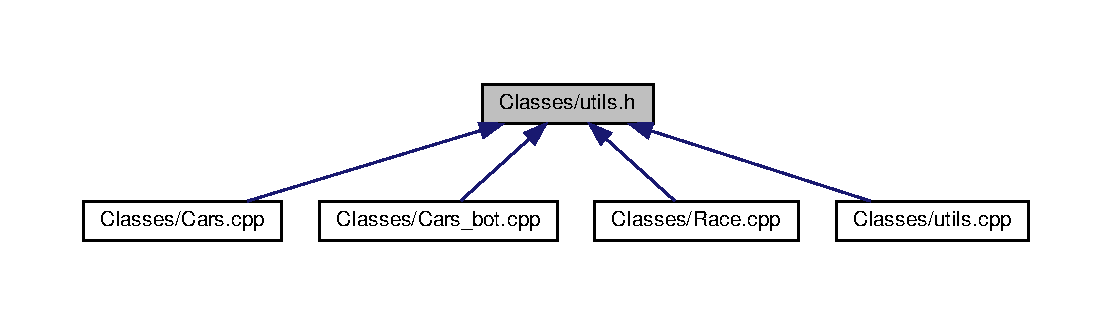
\includegraphics[width=350pt]{utils_8h__dep__incl}
\end{center}
\end{figure}
\subsection*{Classes}
\begin{DoxyCompactItemize}
\item 
class \hyperlink{classutils}{utils}
\end{DoxyCompactItemize}

\hypertarget{_c_make_lists_8txt}{}\section{C\+Make\+Lists.\+txt File Reference}
\label{_c_make_lists_8txt}\index{C\+Make\+Lists.\+txt@{C\+Make\+Lists.\+txt}}

\hypertarget{main_8cpp}{}\section{main.\+cpp File Reference}
\label{main_8cpp}\index{main.\+cpp@{main.\+cpp}}
{\ttfamily \#include \char`\"{}Classes/\+Race.\+h\char`\"{}}\newline
Include dependency graph for main.\+cpp\+:
\nopagebreak
\begin{figure}[H]
\begin{center}
\leavevmode
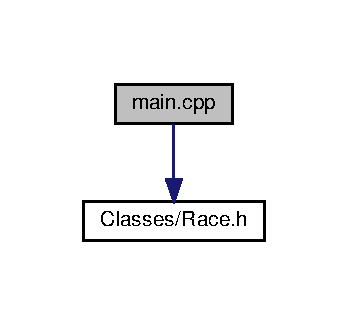
\includegraphics[width=167pt]{main_8cpp__incl}
\end{center}
\end{figure}
\subsection*{Functions}
\begin{DoxyCompactItemize}
\item 
int \hyperlink{main_8cpp_ae66f6b31b5ad750f1fe042a706a4e3d4}{main} ()
\end{DoxyCompactItemize}


\subsection{Function Documentation}
\mbox{\Hypertarget{main_8cpp_ae66f6b31b5ad750f1fe042a706a4e3d4}\label{main_8cpp_ae66f6b31b5ad750f1fe042a706a4e3d4}} 
\index{main.\+cpp@{main.\+cpp}!main@{main}}
\index{main@{main}!main.\+cpp@{main.\+cpp}}
\subsubsection{\texorpdfstring{main()}{main()}}
{\footnotesize\ttfamily int main (\begin{DoxyParamCaption}{ }\end{DoxyParamCaption})}


\hypertarget{_r_e_a_d_m_e_8md}{}\section{R\+E\+A\+D\+M\+E.\+md File Reference}
\label{_r_e_a_d_m_e_8md}\index{R\+E\+A\+D\+M\+E.\+md@{R\+E\+A\+D\+M\+E.\+md}}

%--- End generated contents ---

% Index
\backmatter
\newpage
\phantomsection
\clearemptydoublepage
\addcontentsline{toc}{chapter}{Index}
\printindex

\end{document}
